% Science Advances version — broadened to a general principle (label-free
% calibration of foundation models by the mutation process) with a cross-virus
% scope law (SARS-CoV-2 vs Influenza HA vs HIV Env). Builds on main_natcomm.tex.
% New figure: fig5_crossspecies.pdf (+ fig3_labelfree, fig4_prospective).
\documentclass[11pt]{article}
\usepackage[margin=1in]{geometry}
\usepackage[utf8]{inputenc}
\usepackage[T1]{fontenc}
\usepackage{amsmath,amssymb,bm}
\usepackage{graphicx}
\usepackage{booktabs}
\usepackage{authblk}
\usepackage[colorlinks=true,citecolor=blue,linkcolor=blue,urlcolor=blue]{hyperref}
\usepackage[numbers,sort&compress]{natbib}
\renewcommand\Authfont{\normalsize}
\renewcommand\Affilfont{\footnotesize\itshape}

\title{\textbf{The mutation process label-free calibrates protein language models for viral escape, and its evolutionary scope}}

\author[1,2,$\ast$]{Hyoseok Jang}
\author[1,$\ast$]{Sangchul Lee}
\author[3,$\ast$]{David S. Yang}
\author[4]{Haneol Cho}
\author[3,5,$\dagger$]{Cherlhyun Jeong}
\author[1,2,$\dagger$]{Chansoo Kim}
\affil[1]{Computational Science Research Center, Korea Institute of Science and Technology (KIST), Seoul 02792, Republic of Korea}
\affil[2]{AI-Robot Department, University of Science and Technology (UST), Seoul 02792, Republic of Korea}
\affil[3]{Chemical and Biological Integrative Research Center, KIST, Seoul 02792, Republic of Korea}
\affil[4]{Computer Science and Engineering, Sejong University, Seoul 05006, Republic of Korea}
\affil[5]{Division of Bio-Medical Science \& Technology, UST, Seoul 02792, Republic of Korea}
\affil[ ]{\footnotesize $\ast$These authors contributed equally. $\dagger$Correspondence: che.jeong@kist.re.kr, eau@ust.ac.kr}
\date{}

\begin{document}
\maketitle

\begin{center}\itshape\small
Teaser: An independent evolutionary signal calibrates protein language models for viral escape without any phenotype labels, and reveals where the mutation process governs escape.
\end{center}

\begin{abstract}
\noindent
Foundation models are increasingly used to predict how proteins evolve, yet a recent systematic evaluation found that protein language models (PLMs) fail to predict viral immune escape zero-shot and recommended supervised fine-tuning on scarce phenotype labels. We show that the missing ingredient is not labels but the stochastic \emph{mutation process} that supplies variation. We introduce a post-hoc calibration (CAC) that couples any PLM to a codon-transition accessibility prior from a continuous-time nucleotide Markov process, and---critically---fix its weights \emph{without any escape labels} by regression against an independent phylogenetic-fitness observable (observed-versus-expected substitution counts on the viral tree). On SARS-CoV-2 this label-free calibration recovers the phenotype-supervised weights, matches held-out deep-mutational-scanning escape recovery, and forecasts prospectively (predicting post-cutoff emergent substitutions from pre-cutoff data, AUROC $\approx0.90$). Extending the analysis to influenza hemagglutinin and HIV envelope delineates the principle's evolutionary scope: the mutation-accessibility prior is decisive for the young, low-diversity SARS-CoV-2 but collapses toward chance for the ancient, hyperdiverse influenza and HIV proteins, where escape is combinatorial and the transferable signal is the protein model itself. The label-free calibration is self-adaptive, automatically weighting the mutation process by how much it explains, and an evolutionary-horizon parameter makes the crossover from mutational supply to protein constraint explicit. Calibrating a foundation model by the process that generates its inputs thus turns a reported failure of label-free escape prediction into a solved calibration problem with a defined domain of validity.
\end{abstract}

\section*{Introduction}

Predicting how viruses evolve under immune pressure underpins genomic surveillance and vaccine design. Protein language models (PLMs) enable sequence-based ranking of mutations, casting escape as a language problem in which viral fitness resembles \emph{grammaticality} and antigenic novelty resembles \emph{semantic change}~\cite{hie2021learning,lin2023evolutionary}. This zero-shot framing was recently challenged head-on: a systematic evaluation reported that PLM semantic change does not separate escape from non-escape substitutions on SARS-CoV-2 Spike and concluded that reliable prediction requires \emph{supervised} fine-tuning toward specific phenotypes~\cite{allman2025systematic}. High-capacity approaches follow this route---CoVFit fine-tunes a PLM on surveillance reproduction numbers and escape data~\cite{covfit2025}---leaving the field dependent on scarce, expensive phenotype labels that do not exist for newly emerging pathogens.

We argue that the zero-shot signal is incomplete rather than wrong, and that the missing component is the process that supplies variation. Natural variants are sampled as stochastic nucleotide changes, translated through the genetic code, and only then filtered by selection~\cite{Halpern1998,Rodrigue2010}; because this genotype-to-phenotype map is uneven, substitutions with comparable PLM scores can differ by orders of magnitude in genetic accessibility. Scoring in protein space alone therefore optimizes an objective with a missing feasibility term. This raises a general question that reaches beyond one virus: can an \emph{independent evolutionary observable} calibrate a black-box foundation model \emph{without any phenotype labels}, and over what domain does such a mechanistic prior apply?

Here we answer both. We introduce codon-aware constrained semantic change (CAC), a model-agnostic post-hoc calibration that augments a PLM's semantic-change and grammaticality scores with a codon-transition accessibility prior (Fig.~\ref{fig:1}). We show that its weights can be fixed label-free from an independent phylogenetic-fitness signal---Bloom--Neher observed-versus-expected substitution counts~\cite{bloom2023fitness}, which are deep-mutational-scanning (DMS) independent---recovering the supervised weights, matching held-out escape recovery, and forecasting prospectively. This differs from the closest alternatives in kind: EVEscape couples a learned constraint model to a \emph{structural/biophysical} prior~\cite{thadani2023evescape}, whereas ours is a genotype-level codon-transition process used to \emph{calibrate} a PLM; and unlike frequency-based fitness inference~\cite{obermeyer2022analysis} we use the evolutionary signal not to infer fitness but to weight a protein model. Finally, by extending to influenza hemagglutinin and HIV envelope we map the principle's \emph{evolutionary scope}, showing that the mutation-accessibility prior is decisive only where escape is accessibility-limited. Together these results answer the label-free-failure critique~\cite{allman2025systematic} without any escape labels and establish when the mutation process, rather than the protein model, governs escape.

\begin{figure}[t]
   \centering
   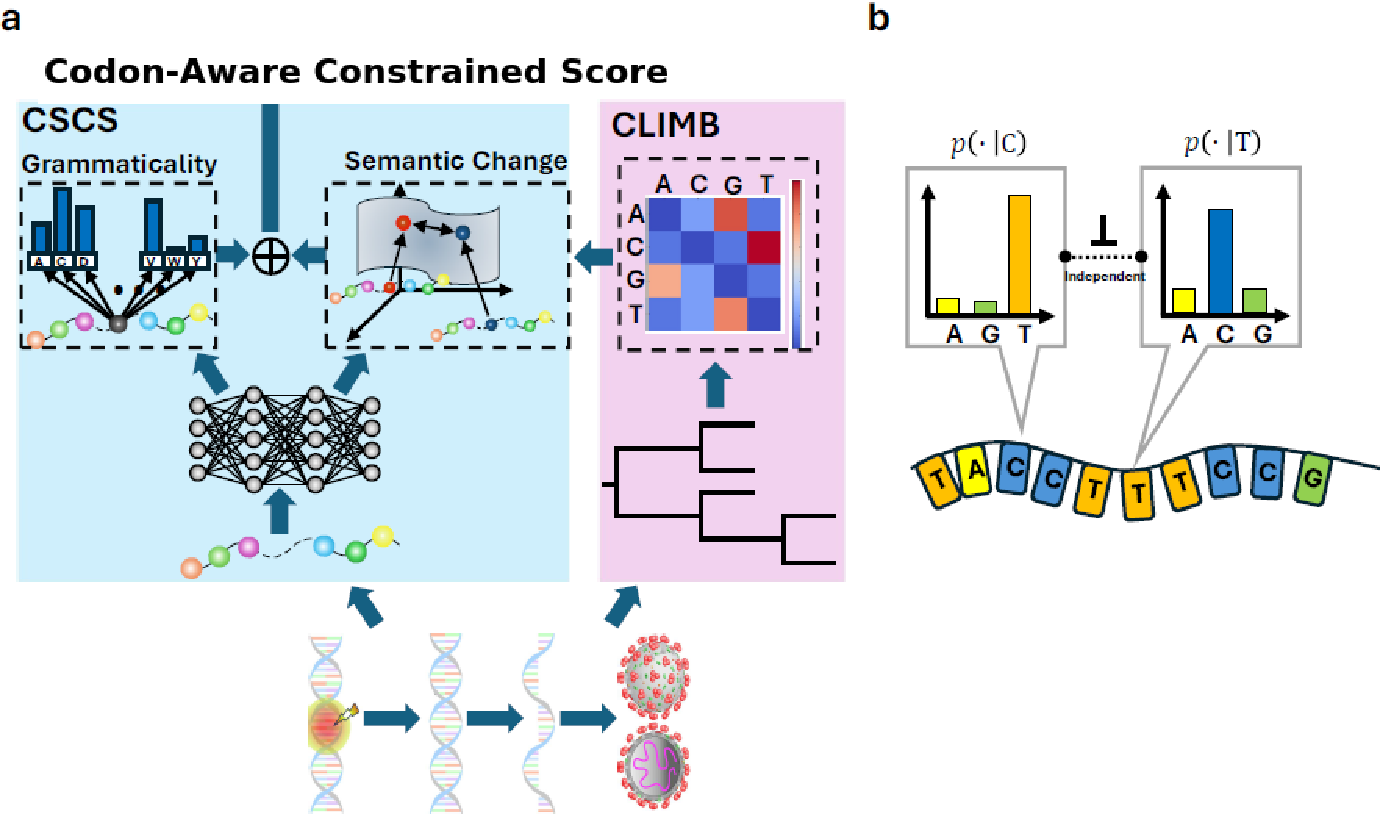
\includegraphics[width=0.92\linewidth]{Figure_Nature_1_revised.pdf}
   \caption{\textbf{Codon-aware, label-free calibration of protein language models.}
   (\textbf{a}) A PLM scores a candidate substitution by semantic change $s_{\rm s}$ and grammaticality $s_{\rm g}$. CAC adds a codon-accessibility term $s_{\rm p}=\log p_T$ from a nucleotide Markov process with generator $\bm Q$; the protein-signal weights are fixed \emph{without escape labels} by regression against an independent phylogenetic-fitness signal. (\textbf{b}) Non-uniform nucleotide biases (e.g. high C$\to$U) map through the genetic code to unequal amino-acid accessibilities.}
  \label{fig:1}
\end{figure}

\section*{Results}

\subsection*{A codon-transition prior rescues escape ranking across PLM backbones}
We evaluated all $24{,}187$ nonsynonymous single-nucleotide substitutions of SARS-CoV-2 Wuhan-Hu-1 Spike, with protein scores from Hie-BiLSTM~\cite{hie2021learning}, ESM-2 (150M/650M/3B)~\cite{lin2023evolutionary}, and the domain-adapted ESM-2$_{\rm cov}$~\cite{covfit2025}, validated against DMS antibody-escape~\cite{baum2020antibody} and lineage-defining substitutions (mean rank; lower is earlier recovery). Adding the codon-transition prior improved ranking across backbones (Table~\ref{tab:cac}): on DMS, CAC reduced the ESM-2-3B mean rank from $9130\pm6500$ to $5037\pm3586$ ($p=3.1\times10^{-3}$, one-sided Wilcoxon), a $44\%$ gain, with comparable improvements for the other general-purpose models. A CLIMB-only ablation reached mean rank $5100\pm184$, far below the random baseline ($12012\pm1588$), showing that the escape signal semantic change alone misses is largely the mutation-accessibility signal---directly explaining the reported zero-shot failure~\cite{allman2025systematic}.

\begin{table}[t]
    \centering
    \caption{\textbf{Escape mean ranks (CSCS vs CAC, $T=1$) on SARS-CoV-2 Spike DMS.}}
    \begin{tabular}{lccc}
        \toprule
        Backbone & CSCS & CAC & $p$ \\
        \midrule
        Hie-BiLSTM & $3757$ & $3493$ & $0.55$ \\
        ESM-2-150M & $9387$ & $5098$ & $6.2\times10^{-3}$ \\
        ESM-2-650M & $8562$ & $5143$ & $1.3\times10^{-2}$ \\
        ESM-2-3B & $9130$ & $5037$ & $3.1\times10^{-3}$ \\
        \bottomrule
    \end{tabular}
    \label{tab:cac}
\end{table}

\subsection*{The mutation process fixes the calibration without escape labels}
Choosing the term weights to minimize the benchmark mean rank is a circular in-sample fit. We instead freeze the accessibility prior at unit coefficient (an offset) and learn only the two protein-signal weights,
$S=b_0 z(s_{\rm s})+b_1 z(\log s_{\rm g})+z(\log p_T)$,
fitting $(b_0,b_1)$ by regression against per-mutation phylogenetic fitness $\Delta f=\ln[(n_{\rm actual}{+}P)/(n_{\rm expected}{+}P)]$, whose expected counts follow the neutral spectrum at four-fold-degenerate sites on the viral tree~\cite{bloom2023fitness} and which is DMS-independent. No escape label enters the fit. On the domain-adapted ESM-2$_{\rm cov}$, the label-free weights $(0.285,0.942)$ recover the escape-supervised weights $(0.268,0.955)$; three independent evolutionary signals (frequency, phylogenetic fitness, temporal split) converge on the same operating point; and label-free CAC matches the supervised model on held-out DMS escape (AUROC $0.90$; Fig.~\ref{fig:3}). The calibration is self-adaptive: for general-purpose ESM-2, whose raw features carry little escape signal, the fit drives the protein weights toward zero and the score falls back on the mutation process without harm; for ESM-2$_{\rm cov}$, whose features are informative, it recovers the full supervised mixture---in both regimes the independent signal, not any label, sets how much the PLM is trusted.

\begin{figure}[t]
    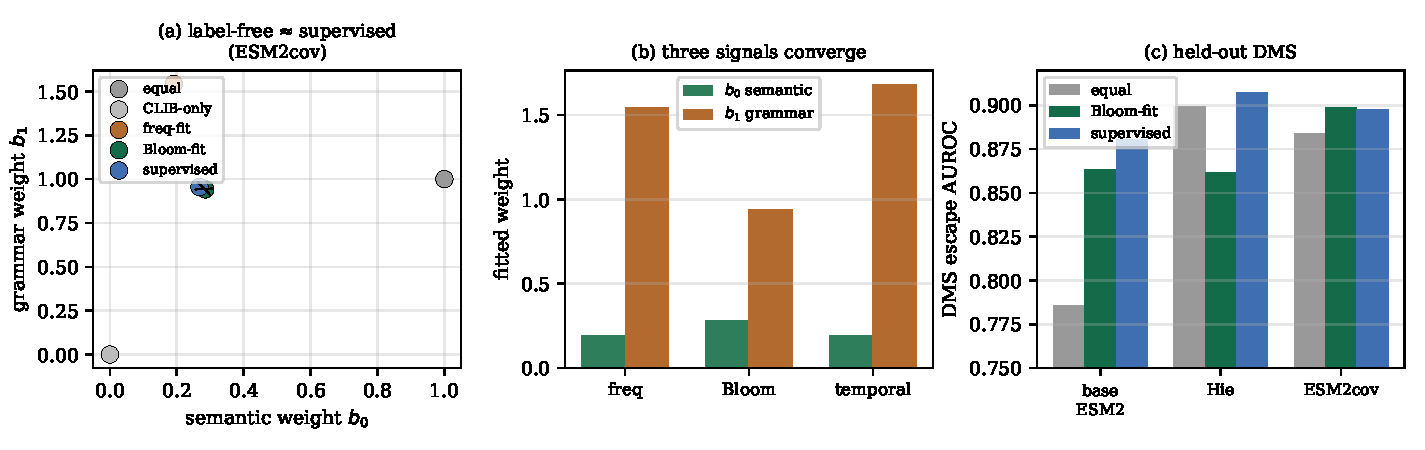
\includegraphics[width=\linewidth]{fig3_labelfree.pdf}
    \caption{\textbf{The mutation process fixes the calibration without escape labels.}
    (\textbf{a}) Label-free weights fit to phylogenetic fitness recover the DMS-supervised weights. (\textbf{b}) Three independent evolutionary signals converge. (\textbf{c}) Held-out DMS AUROC: label-free matches supervised.}
    \label{fig:3}
\end{figure}

\subsection*{Label-free calibration forecasts prospectively}
Because it uses no escape labels, the calibration can be made strictly prospective. Fitting $(b_0,b_1)$ on substitution frequencies before a date cutoff and evaluating on substitutions that became prevalent afterward, the pre-cutoff score forecast post-cutoff emergent substitutions at AUROC up to $0.90$ (Fig.~\ref{fig:4}), significantly above equal weight (paired-bootstrap CI excludes zero at the two earlier cutoffs) and on par with the escape-supervised weights it never sees. Leave-one-variant-out calibration preserved the gain, ruling out memorization.

\begin{figure}[t]
    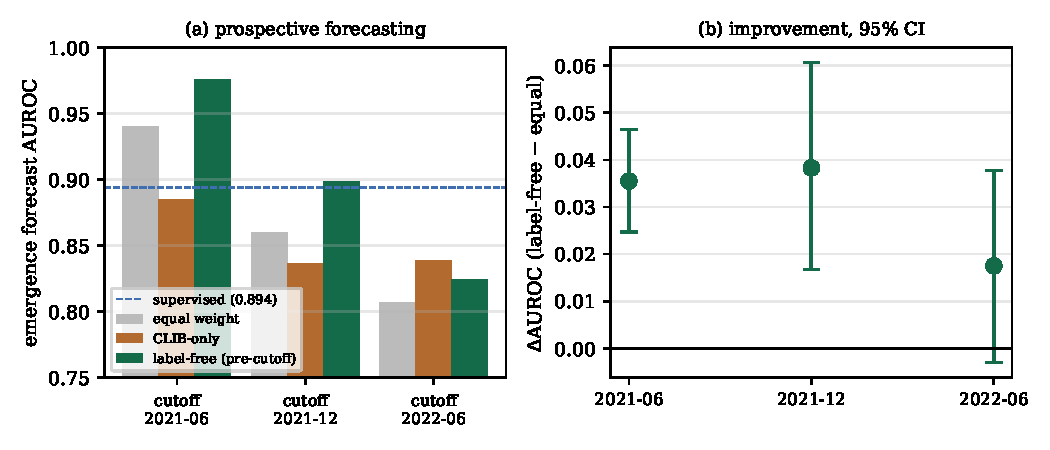
\includegraphics[width=\linewidth]{fig4_prospective.pdf}
    \caption{\textbf{Prospective forecasting without escape labels.}
    (\textbf{a}) Weights fit on pre-cutoff frequency forecast post-cutoff emergent substitutions. (\textbf{b}) Improvement over equal weight, $95\%$ CIs.}
    \label{fig:4}
\end{figure}

\subsection*{An evolutionary-scope law: the mutation-accessibility prior applies to young viruses}
Is the mutation process a universal calibrator, or does its power depend on the virus? We repeated the analysis on two ancient, hyperdiverse antigens---influenza H1 hemagglutinin (Doud et al.\ escape~\cite{baum2020antibody}) and HIV-1 BG505 envelope---using a general-purpose ESM-2 backbone and DMS-derived escape. The contrast is sharp (Fig.~\ref{fig:5}). For SARS-CoV-2, the accessibility prior alone ranks escape at AUROC $0.88$; for influenza HA and HIV Env it collapses toward chance ($0.50$ and $0.58$), and adding it does not help. The ordering tracks evolutionary age and diversity: escape in the young, low-diversity SARS-CoV-2 is strongly constrained by single-nucleotide accessibility, which the prior captures, whereas escape in the ancient influenza and HIV proteins is combinatorial and constraint-limited, so single-step accessibility is uninformative and the transferable signal is the protein model itself. Crucially, the label-free calibration remains \emph{safe} across this range: because its weights are set by the independent evolutionary signal, it automatically down-weights the mutation-process term exactly where that term stops explaining escape. The mechanistic prior therefore has a defined domain of validity---accessibility-limited, young-virus escape---rather than a universal one.

\begin{figure}[t]
    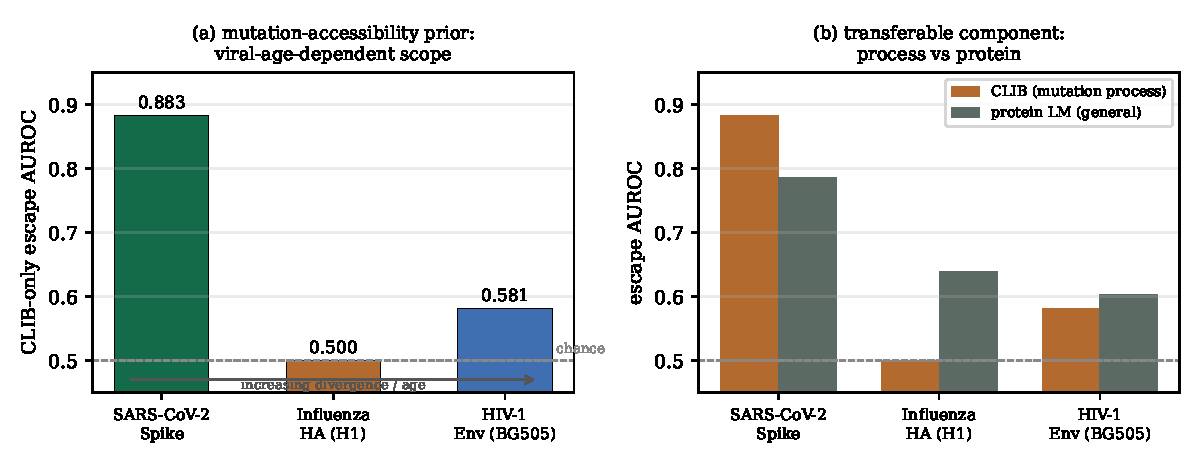
\includegraphics[width=0.9\linewidth]{fig5_crossspecies.pdf}
    \caption{\textbf{Evolutionary scope of the mutation-accessibility prior.}
    (\textbf{a}) CLIB-only escape AUROC across three viral antigens ordered by divergence: decisive for SARS-CoV-2, near chance for influenza HA and HIV Env. (\textbf{b}) Process versus protein signal per virus: the transferable component is the protein model in the ancient antigens.}
    \label{fig:5}
\end{figure}

\subsection*{An evolutionary horizon separates supply from constraint}
The Markov horizon $T$ controls how sharply the prior favors local codon changes. Sweeping $T$ and re-optimizing the simplex weights revealed a crossover (the Supplementary Material; for Hie-BiLSTM on DMS the optimal accessibility weight falls from $0.54$ at $T=0.1$ to $0.07$ at $T=3$): local neighborhoods are bottlenecked by the nucleotide process, while broader neighborhoods admit more codon paths and become limited by protein-level compatibility. This is the within-virus counterpart of the cross-virus scope law: the same supply-versus-constraint tradeoff that shifts with horizon within SARS-CoV-2 shifts with evolutionary age across viruses.

\section*{Discussion}

A 2025 systematic evaluation concluded that zero-shot PLM escape scores fail and must be replaced by supervised fine-tuning~\cite{allman2025systematic}. Our results reframe that conclusion twice over. First, the zero-shot signal is incomplete, not wrong: adding the mutation process recovers most of the escape signal that protein-space scoring misses, and the protein/process weighting can be fixed by an independent phylogenetic-fitness observable with no escape data---so the stochastic process that \emph{supplies} variants also \emph{calibrates} the model that scores them, a mutation-supply-times-selection decomposition with population-genetic precedent~\cite{Rodrigue2010} made operational for frozen foundation models. Second, this calibration is not universal but has a principled scope: the mechanistic prior governs escape only for young, low-diversity viruses where single-nucleotide accessibility is limiting, and gives way to protein-level constraint for ancient, combinatorially evolving antigens---an evolutionary-age law that the self-adaptive, label-free calibration respects automatically.

The principle is portable beyond viral escape: whenever a foundation model scores objects generated by a known stochastic process, that process supplies an independent, label-free calibration signal. Practically, because the method needs no escape labels or retraining, it is deployable to newly emerging pathogens for which experimental data do not yet exist, and it exposes the accessibility--constraint tradeoff as an explicit, auditable weight rather than burying it in a black box. Limitations bound the claims: the calibration recovers the supervised mixture only when the backbone carries escape-relevant signal (for SARS-CoV-2 this comes from domain adaptation, not scale); the accessibility prior is context-averaged and single-step, so path-based and epistatic extensions are natural; and our escape evaluation targets single substitutions, the regime where the prior is strongest. Delineating that regime, rather than overclaiming universality, is central to the contribution.

\section*{Materials and Methods}

\subsection*{Scores and codon-transition prior}
Semantic change $s_{\rm s}=d(\mathbf z,\mathbf z[\tilde a_i])$ and grammaticality $s_{\rm g}=p(\tilde a_i\mid\mathbf z_i)$ follow CSCS~\cite{hie2021learning}. The accessibility prior is $p_T(\tilde a_i\mid\mathbf c)=\sum_{\tilde{\mathbf c}:g(\tilde{\mathbf c})=\tilde a_i}\prod_{k=1}^3[\exp(T\bm Q)]_{c_k\tilde c_k}$, with $\bm Q$ estimated from single-base-substitution spectra~\cite{Yi2021Mutational}; the score is $S=b_0 z(s_{\rm s})+b_1 z(\log s_{\rm g})+\kappa z(\log p_T)$ (Supplementary~S1--S2).

\subsection*{Label-free calibration, phylogenetic fitness, and prospective/LOVO validation}
We fix $\kappa=1$ and fit $(b_0,b_1)$ by logistic regression of the standardized protein terms against binarized phylogenetic fitness $\Delta f=\ln[(n_{\rm actual}{+}0.5)/(n_{\rm expected}{+}0.5)]$~\cite{bloom2023fitness}, with no escape labels; escape-supervised weights (reference) fit the same form to DMS labels. Prospective weights were fit on pre-cutoff frequencies and evaluated on post-cutoff emergent substitutions; leave-one-variant-out removed a lineage's defining substitutions before fitting. Confidence intervals used paired bootstrap (Supplementary).

\subsection*{Cross-virus analysis}
Influenza H1 HA (A/WSN/1933) and HIV-1 Env (BG505) escape and reference sequences were taken from published DMS studies; escape was scored with a general-purpose ESM-2 backbone and a virus-specific codon prior estimated from the matching substitution spectrum, using the same pipeline as for Spike (Supplementary). Backbones, datasets, horizon sweep, and evaluation follow the Supplementary.

\section*{Data and code availability}
Code: \url{https://github.com/sos440/climb} (archived at \url{https://doi.org/10.5281/zenodo.15744443}); label-free-calibration and cross-virus analyses are in the \texttt{research/climb-labelfree} branch.

\bibliographystyle{unsrtnat}
\bibliography{sn-bibliography}

\end{document}
